% Copyright 2013 Nicolai Hähnle <nhaehnle@gmail.com>
%
% This work is licensed under the Creative Commons Attribution-ShareAlike 3.0
% Unported License, see http://creativecommons.org/licenses/by-sa/3.0/
%
% Among other things, this means that yes, you may take e.g. illustrations from
% the book and use them in your own work. However, (a) you must give proper
% attribution by naming me as its original author and (b) you must make your
% derivative work available under the same or similar license terms.
%
% See the Creative Commons website for the exact licensing terms.

\chapter{Lattice programming}

We now consider the problem of deciding whether a given convex body $K \subset \R^d$
contains a point from a lattice $\Lambda \subset \R^d$.
As was already hinted at in the previous chapter,
the Flatness Theorem plays a crucial role in this problem.
We have seen that if the lattice width of $K$ is large,
then the answer is ``yes'': $K$ does contain a lattice point.
On the other hand,
if the lattice width of $K$ is small,
then recursing into all lattice hyperplanes that intersect $K$ is not too bad.
The resulting recursion tree can still be quite large:
if our bound on the lattice width is $d^c$ when we recurse,
then the number of leaves is bounded from above by
\[
  d^c \cdot (d-1)^c \cdots 2^c = 2^{O(d \log d)},
\]
which will dominate the running time of our algorithm.
Indeed, it is an important open research problem
whether the lattice programming problem can be decided
with a running time whose dependence on $d$ is only $2^{O(d)}$.

How does one determine the lattice width of $K$?
In the previous chapter,
we have seen that we can get an approximation if we approximate $K$ by its Löwner-John ellipsoid.
This ellipsoid can be approximated efficiently using linear programming techniques,
and we could use such approximations as a black box.
However, there is a slight technical issue:
if $K$ is given by a separation oracle rather than explicitly,
then all black box algorithms require some knowledge about the minimum volume of $K$.
To sidestep this issue,
we will follow an approach in which the
ellipsoid method and lattice programming recursion are integrated in a single algorithm.

Throughout this chapter, we will assume that we can perform basic operations, including square roots,
on real numbers in constant time.
This is obviously a simplification,
since ironically one does not compute with reals on real computers.
In reality, the algorithms outlined in this chapter would be implemented using approximations with rational numbers.
It turns out that this can be done without loss of correctness and within essentially the same asymptotic running time.
However, those details tend to become highly technical, and we avoid them for clarity of presentation.



\section{Separation and the half-ball lemma}

We assume that convex bodies $K \subset \R^d$ are given by an enclosing ellipsoid $E \supset K$
and access to a \emph{separation oracle}.
The separation oracle is a black box algorithm which, given $z \in \R^d$,
tells us whether $z \in K$.
Furthermore, if $z \not\in K$, it returns a separating hyperplane $a^Tx \leq \beta$.
We assume that each call to the oracle takes constant time,
see Figure~\ref{fig:separating-hyperplane}.
\begin{figure}
  \begin{center}
    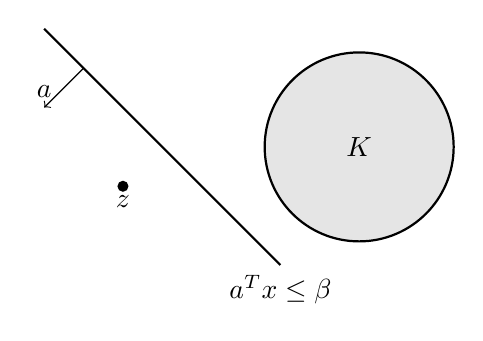
\begin{tikzpicture}
      \fill (0,0) circle[radius=2pt] node[below] {$z$};

      \draw[thick,fill=black!10] (3,0.5) node {$K$} circle[radius=1.2cm];

      \draw[thick] (2,-1) node[below] {$a^Tx \leq \beta$} -- (-1,2);
      \draw[->] (-0.5,1.5) -- +(-0.5,-0.5) node[above] {$a$};
    \end{tikzpicture}
  \end{center}
  \caption{A separating hyperplane exists for every $z \not\in K$.}
  \label{fig:separating-hyperplane}
\end{figure}

\begin{remark}
  In fact, analogous results can be achieved even if $K$ is only given by a \emph{weak} separation oracle,
  where some imprecision is allowed in the oracle for points close the boundary of $K$.
  In this case, most of the analysis can proceed as if the oracle were in fact supplying the answer
  for a convex body $K'$ that is only slightly different from $K$.
  We will ignore such details to keep the presentation simple.
\end{remark}

We are given an ellipsoid $E \supset K$.
In fact, we can assume that $E$ is a ball with center $z'$
by applying the same linear transformation to $E$, $K$, and $\Lambda$.
We can now compute a closest vector $z \in \Lambda$ to $z'$ as a candidate lattice point
in time $2^{O(d)} \poly(b)$.
If $z \not\in E$, we can conclude that $K$ contains no lattice point.
Otherwise, we can feed $z$ into the separation oracle for $K$.
If $z \in K$, we are done.

Otherwise, if $z \not\in K$,
we obtain a linear inequality $a^Tx \leq \beta$ that separates $z$ from $K$.
In fact, the inequality splits $E$ into two parts,
and we are guaranteed that $K$ is entirely contained in one of them.
We will now compute a new ellipsoid $E'$ that contains this second part,
see Figure~\ref{fig:ellipsoid-method}.
\begin{figure}
  \begin{center}
  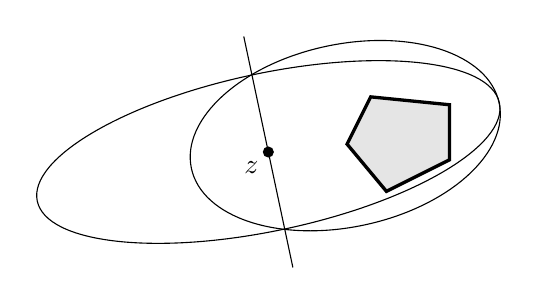
\begin{tikzpicture}
    \fill (0,0) circle [radius=2pt];
    \draw (0,0) node[below left] {$z$};

    \draw[very thick,fill=black!10] (1,0.1) -- (1.3,0.7) -- (2.3,0.6) -- (2.3,-0.1) -- (1.5,-0.5) --cycle;

    \begin{scope}[rotate=12,xscale=3]
      \draw (0,0) circle [x radius=1,y radius=1];
      \draw (0,-1.5) -- (0,1.5);
      \draw (0.333,0) circle [x radius=0.666,y radius=1.16];
    \end{scope}
  \end{tikzpicture}
  \end{center}
  \caption{Computing a tighter ellipsoid containing $K$.}
  \label{fig:ellipsoid-method}
\end{figure}

To simplify the argument,
assume first that $E$ is a unit ball centered at the origin
and the linear equality is $x_1 \geq -\eta$ with $\eta \geq 0$.
This can always be achieved by an affine transformation of $E$ and possibly by shifting the hyperplane
so that the enclosed part of $E$ becomes larger.
By symmetry, the smallest volume ellipsoid containing $E \cap \{ x_1 \geq -\eta \}$ is of the form:
\[
  E' = \{ x \in \R^d ~:~ \alpha^2 (x_1 - c)^2 + \beta^2 (x_2^2 + \dots + x_d^2) \leq 1 \}
\]
Intuitively, we expect $\alpha > 1$ and $\beta < 1$ so that $E'$ results from the unit ball
by compressing it in the $x_1$ direction and scaling it in the other directions.
The centroid of $E'$ is at $(c,0,\ldots,0)$.

The point $x_1$ should lie on the boundary of $E'$, which implies:
\[
  \alpha^2 (1-c)^2 = 1 \quad\implies\quad \alpha^2 = \frac{1}{(1-c)^2}
\]
Furthermore, the sphere $\partial E \cap \{ x_1 = -\eta \}$ should also lie on the boundary of $E'$.
For points in this set, one has
\[
  x_2^2 + \dots + x_d^2 = 1 - \eta^2,
\]
and hence we obtain the condition
\[
  \alpha^2 (c + \eta)^2 + \beta^2 (1 -\eta^2) = 1
\]
on the parameters of $E'$.
We can solve for $\beta^2$:
\begin{align*}
  \beta^2
    &= \frac{1}{1 - \eta^2} \left( 1 - \frac{(c+\eta)^2}{(1-c)^2} \right) \\
    &= \frac{(1-c)^2 - (c+\eta^2)}{(1-c)^2 (1-\eta^2)} \\
    &= \frac{1-2c - 2c\eta - \eta^2}{(1-c)^2 (1-\eta)(1+\eta)} \\
    &= \frac{(1-\eta)(1+\eta) - 2c(1 + \eta)}{(1-c)^2 (1-\eta)(1+\eta)} \\
    &= \frac{(1-\eta) - 2c}{(1-c)^2 (1-\eta)}
\end{align*}
Now that we have expressed both $\alpha$ and $\beta$ in terms of $c$,
observe that
\[
  \left(\frac{\vol(E)}{\vol(E')}\right)^2 = \alpha^2 (\beta^2)^{d-1} = \frac{(\kappa - 2c)^{d-1}}{(1-c)^{2d} \kappa^{d-1}} = \frac{(1 - \frac{2c}{\kappa})^{d-1}}{(1-c)^{2d}},
\]
where $\kappa = 1 - \eta$.
We want this fraction to be as large as possible,
so that the volume of $E'$ is minimal.
Let us compute the derivative with respect to $c$:
\[
  2d \frac{(1 - \frac{2c}{\kappa})^{d-1}}{(1-c)^{2d+1}} - \frac{(d-1) \frac{2}{\kappa} (1-\frac{2c}{\kappa})^{d-2}}{(1-c)^{2d}}
\]
We set this quantity to $0$ and simplify
\begin{align*}
  2d\frac{1-\frac{2c}{\kappa}}{1-c} &= \frac{2(d-1)}{\kappa}
\end{align*}
and eventually obtain:
\[
  c = \frac{1 - \eta d}{d + 1}
\]
Note how a larger $\eta$ means that the centroid of $E'$ moves closer to the origin.
Intuitively, this means that $E'$ approaches the unit ball,
and we do not get a genuinely new ellipsoid if $\eta > \frac{1}{d}$.
Still, we do obtain the following result:

\begin{lemma}
  Let $E \subseteq \R^d$ be an ellipsoid and let
  $a^Tx \leq \beta$ be an inequality such that $a^Tx \geq \beta$ for some point of $\eta \star E$ for some $\eta \leq \frac{1}{2d}$.
  Then there exists an ellipsoid $E' \supset E \cap \{ x ~:~ a^Tx \leq \beta \}$
  with $\vol(E') \leq \vol(E) ...$.
\end{lemma}
\begin{proof}
  The condition on $\eta \star E$ ensures that a linear transformation can be used to reduce the problem to the setting we just discussed.
  The ellipsoid compute above satisfies
  \begin{align*}
    \frac{\vol E'}{\vol E} = \alpha^{-1} \beta^{-{d-1}}
  \end{align*}
\end{proof}













